
\documentclass[a4paper,10pt]{article}
\usepackage{graphics,color,amsfonts,amssymb,amsmath,pgf,xcolor}
\usepackage{graphicx,tikz}
\newcommand{\comment}[1]{}




\title{AUTOINSERT}
\author{Benny George K}
\date{\today }

\begin{document}

\maketitle

Consider the  graph $G$ shown in Fig 1. and the word $aebacfdbce$.
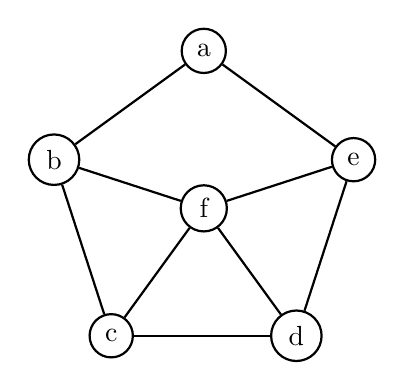
\begin{tikzpicture}[thick]

% Define nodes with polar coordinates in a loop
\foreach \name/\radius/\angle in {a/2/90, b/2/162, c/2/234, d/2/306, e/2/18} {
    \node[circle, draw] (\name) at ({\radius*cos(\angle)}, {\radius*sin(\angle)}) {\name};
}

\node[circle,draw] (f) at (0,0) {f};
% Define edges in a loop
\foreach \source/\dest in {a/b,b/c,c/d,d/e,e/a, f/b, f/c, f/d,f/e} {
	  \draw (\source) -- (\dest);
}

\end{tikzpicture}

\bibliographystyle{plain}
\bibliography{/home/ben/Work/bibtex/mybib.bib}
\end{document}

%%% Local Variables:
%%% mode: latex
%%% TeX-master: t
%%% End:
